% --------------------------------------------------------------------------
% Version 3.0
% This template is available on the sites:
% https://www.overleaf.com/read/rpkkfchcnbsc
% https://www.overleaf.com/latex/templates/itmo-beamer-theme/fpttrgnmqwsb
% https://github.com/AlexZabashta/ITMO-Beamer-theme
% --------------------------------------------------------------------------

% Attention!!!
% This document was created only as an example of using ITMO beamer styling.
% Don't use it as a Latex or beamer tutorial!
% Check out the capabilities of Latex and beamer (at least basic) independently.


\documentclass[aspectratio=169]{beamer}
\usepackage{ITMOtheme}
\setbeamercovered{dynamic}

\usepackage{tikz}
\usepackage{pgfplots}
\pgfplotsset{compat=1.18}

% Use this package to automatically format references.
% \usepackage[style=mla]{biblatex}
% \addbibresource{references.bib}

\usepackage{animate}


% The fields 'title', 'author', 'subject', 'keywords' are used to generate a PDF document.
% It is recommended that you fill them in, even if you are creating your title slide manually.

% use \title[short title]{full title}
\title[Counter Strike Reversing \& Anti Cheat]{Game Beneath the Game: The Evolution of Cheats and Anti-Cheat Systems in Counter-Strike 2}

%\subtitle[short subtitle]{long subtitle}

\author[LastName F.]{FirstName LastName}

%\institute[short institute]{long institute}

\where{Madrid}
\date{\today}


\begin{document}


\AtBeginSection[]{
    \begin{frame}
        \frametitle{Outline}
        \tableofcontents[
            currentsection,
            sectionstyle=show/shaded,
            hideothersubsections
        ]
    \end{frame}
}

% Title slide
\begin{frame}[plain,noframenumbering]
    \itmobackgroundsnakes{
        \vfill
        \begin{center}
            \vspace{2cm}
            
            {\usebeamerfont{title}\LARGE\textbf{``The Game Beneath the Game:\\The Evolution of Cheats and Anti-Cheat Systems in Counter-Strike 2''}}\\[1.5em]
            
            \textbf{Author:} Pablo Valiente\\[0.5em]
            \textbf{Supervisor:} Dr. Antonio Nappa\\[3em]
            \textbf{Universidad Carlos III de Madrid}\\[1em]
            \textbf{Academic Year:} 2024--2025\\[0.5em]
        \end{center}
        \vfill
    }
\end{frame}

% Full outline slide
\begin{frame}
    \frametitle{Outline}
    \tableofcontents
\end{frame}


% --- Motivation and Context ---
\section{Motivation and Context}
\begin{frame}
    \frametitle{Motivation}
    My interest in this topic began around six years ago, driven by a passion for competitive video games.
    \vspace{0.4cm}
    \begin{itemize}
        \item \textbf{Curiosity:} Encountering cheaters in ranked matches often led me to wonder: \textit{“How did they do it?”}
        \pause
        \item \textbf{Exploration:} This question gradually introduced me to reverse engineering, memory analysis, and anti-cheat evasion.
        \pause
        \item \textbf{Objective:} To merge this journey with an academic study by analyzing and implementing real cheats to test detection systems.
    \end{itemize}
\end{frame}



% --- New Introductory Slides: Cheating Phenomenon ---

% --- Cheating: History, Ecosystem, and Ethics ---
\section{The Evolution of Cheating: History, Ecosystem, and Ethics}
\begin{frame}
    \frametitle{Understanding Cheating in Online Games}
    Cheating undermines fairness and security in competitive online games.
    \vspace{0.4cm}
    \begin{itemize}
        \item \textbf{Definition:} Any software or hardware manipulation that grants unfair advantage.
        \pause
        \item \textbf{Anti-Cheat:} Monitors and enforces integrity at runtime, acting like an \textbf{EDR} by detecting anomalous behavior, unauthorized memory access, or code injection in protected processes.
        \pause
        \item \textbf{Spectrum:} From basic aimbots to advanced GUI Drawings.
 
    \end{itemize}
\end{frame}

\begin{frame}
    \frametitle{Historical Origins: From Developer Shortcuts to Cheating Tools}
    Cheating emerged from tools meant for testing and evolved into manipulation.
    \vspace{0.4cm}
    \begin{itemize}
        \item \textbf{Debug Codes:} Became public cheat codes (e.g., Konami Code).
        \pause
        \item \textbf{GameShark:} Modified RAM directly on console hardware.
        \pause
        \item \textbf{Cheat Engine \& ReClass.NET:} Allowed advanced memory mapping, pointer tracing, and class reconstruction.
    \end{itemize}
\end{frame}

\begin{frame}
    \frametitle{From Hacks to Services: The Turning Point}
    The early 2010s marked a major shift in how cheats were created, distributed, and perceived.
    \vspace{0.4cm}
    \begin{itemize}
        \item \textbf{Community Forums:} Platforms like UnKnoWnCheaTs fostered knowledge sharing and tutorials.
        \pause
        \item \textbf{Subscription Models:} Private cheats became commercialized with regular updates and support.
    \end{itemize}
    \vspace{0.5cm}
    \only<2->{%
        \begin{center}
            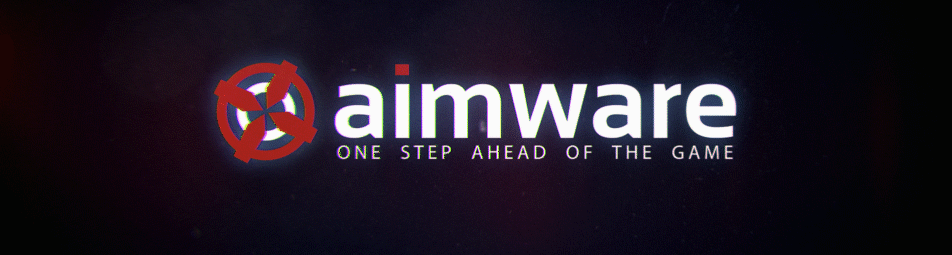
\includegraphics[width=0.6\linewidth]{images/aimware_logo.png}
        \end{center}
    }
\end{frame}

\begin{frame}
    \frametitle{Cheating Today: A Professionalized Ecosystem}
    Cheating has evolved from hobbyist tools to a mature ecosystem that mirrors legitimate software development.
    \vspace{0.4cm}
    \begin{itemize}
        \item \textbf{Commercialization:} Cheat providers operate like startups, offering licensing, tiered features, and customer support.
        \pause
        \item \textbf{Infrastructure:} Loaders, obfuscators, HWID spoofers, and encrypted update channels ensure persistence.
    \end{itemize}
\end{frame}



% --- Anti-Cheat Technologies and Milestones ---
\section{Counter-Strike 2: A Case Study in Cheating Dynamics}



% --- NEW: CS2 Player Base Growth Slide ---
\begin{frame}
    \frametitle{Why Counter Strike 2?}
    To contextualize the scale of CS2's ecosystem, the following graph illustrates the evolution of its player base based on SteamCharts data.
    \vspace{0.3cm}
    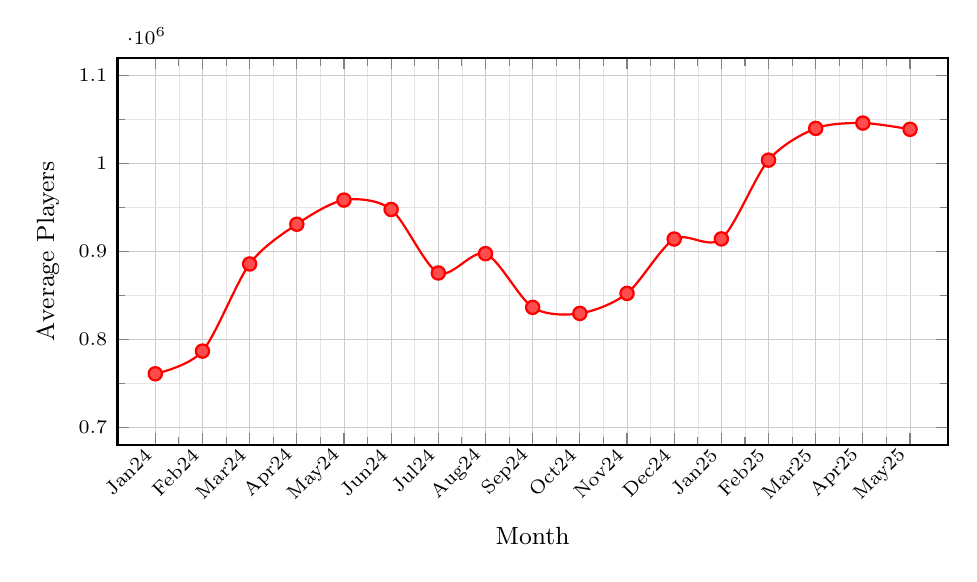
\begin{tikzpicture}
    \begin{axis}[
        width=\linewidth,
        height=6.5cm,
        xlabel={Month},
        ylabel={Average Players},
        symbolic x coords={Jan24, Feb24, Mar24, Apr24, May24, Jun24, Jul24, Aug24, Sep24, Oct24, Nov24, Dec24, Jan25, Feb25, Mar25, Apr25, May25},
        xtick=data,
        xticklabel style={rotate=45, anchor=east, font=\scriptsize},
        yticklabel style={font=\scriptsize},
        label style={font=\small},
        tick style={thin},
        grid=both,
        minor tick num=1,
        major grid style={line width=.3pt, draw=gray!40},
        minor grid style={line width=.2pt, draw=gray!20},
        ymin=700000, ymax=1100000,
        enlargelimits=0.05,
        smooth,
        mark options={scale=1.2, fill=red!70},
        line width=0.8pt,
        legend style={at={(0.5,-0.2)}, anchor=north, font=\small},
    ]
    \addplot[
        color=red,
        mark=*,
    ]
    coordinates {
        (Jan24,760859) (Feb24,786631) (Mar24,885630) (Apr24,930749)
        (May24,958207) (Jun24,947521) (Jul24,875365) (Aug24,897338)
        (Sep24,836307) (Oct24,829439) (Nov24,852164) (Dec24,913953)
        (Jan25,914092) (Feb25,1003571) (Mar25,1039663) (Apr25,1045702)
        (May25,1038597)
    };
    \end{axis}
    \end{tikzpicture}
\end{frame}



% --- NEW: Steam Top 10 Visual Context Slide ---
\begin{frame}
    \frametitle{Steam Top 10: July 7, 2025}
    \begin{center}
        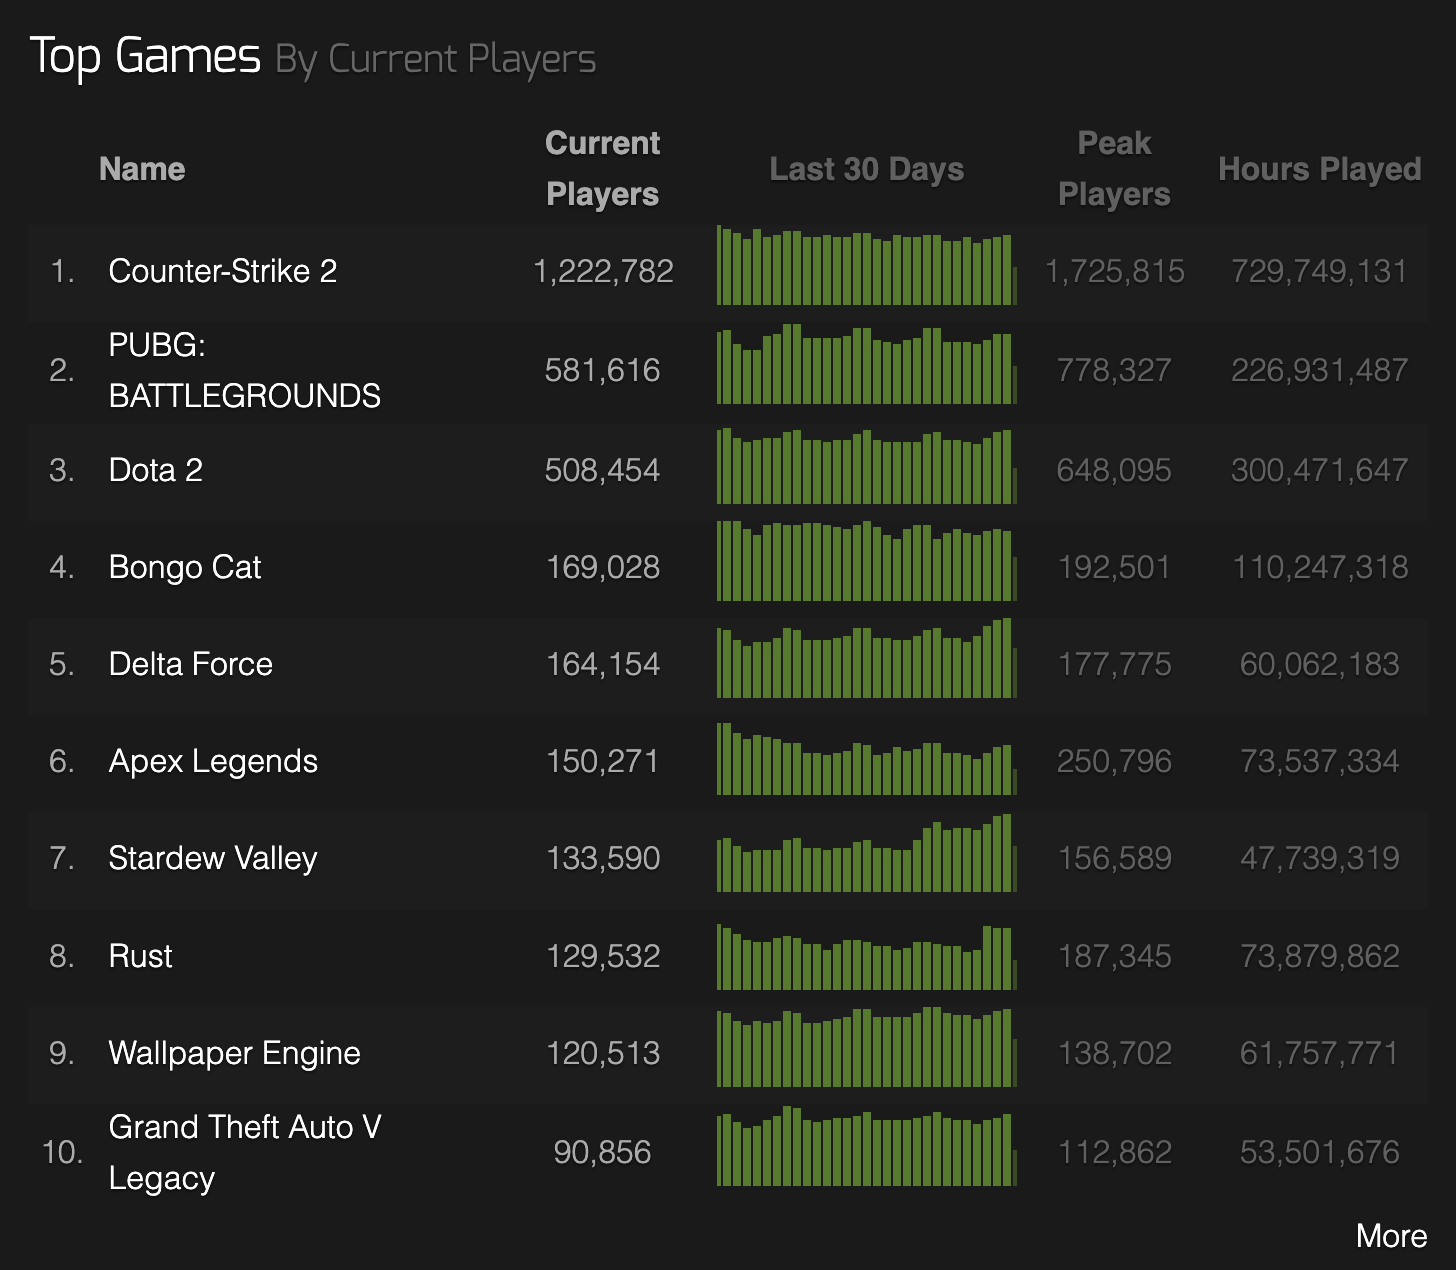
\includegraphics[width=0.63\linewidth]{images/steam_stats.png}
    \end{center}
    \vspace{0.3cm}
\end{frame}


\begin{frame}
    \frametitle{Anti-Cheat Systems Timeline}
    Anti-cheat systems have evolved from basic client-side tools to complex, kernel-level detectors. Each marked a significant shift in visibility, access, or enforcement.
    \vspace{0.4cm}
    \begin{table}[]
        \small
        \begin{tabular}{|l|l|l|l|}
            \hline
            \textbf{System} & \textbf{Year} & \textbf{Mode} & \textbf{Milestone or Innovation} \\
            \hline
            PunkBuster & 2000 & User & First real-time memory scan and screenshot system \\
            VAC & 2002 & User & Delayed ban model to obfuscate detection methods \\
            BattleEye & 2004 & Kernel & Early adoption of kernel-mode drivers \\
            FairFight & 2012 & Server & Behavioral/statistical detection at server level \\
            EAC & 2018 & Kernel & Real-time scanning with driver-level protection \\
            Vanguard & 2020 & Kernel & Persistent always-on kernel driver (controversial) \\
            VAC Live & 2023 & Hybrid & Real-time detection with low-latency enforcement \\
            \hline
        \end{tabular}
    \end{table}
\end{frame}



\section{Code Injection and Cheat Delivery Mechanisms}


\begin{frame}
    \frametitle{VAC Detection and Countermeasures}
    VAC employs both traditional and modern mechanisms to detect unauthorized modifications within the game environment.
    \vspace{0.4cm}
    \begin{itemize}
        \item \textbf{Detection Vectors:} Signature scanning, analysis of suspicious thread start addresses, and detection of VMT (Virtual Method Table) hooks are among its key strategies.
        \pause
        \item \textbf{Steamservice.dll:} Inspection of \texttt{steamservice.dll} reveals that VAC dynamically streams detection modules from Valve’s servers into memory at runtime.
        \pause
        \item \textbf{Dumper Feasibility:} With moderate reverse engineering effort, it is possible to create a dumper capable of capturing and writing these modules to disk for offline analysis.
    \end{itemize}
\end{frame} 

% --- NEW: Survey Slide: Cheating as a Critical Threat ---
\begin{frame}
    \frametitle{Survey: Cheating as a Critical Threat}
    A 2018 global survey by Irdeto revealed the widespread negative impact of cheating in Counter-Strike:
    \vspace{0.4cm}
    \begin{table}[]
        \small
        \centering
        \begin{tabular}{|p{7.5cm}|c|}
            \hline
            \textbf{Survey Statement} & \textbf{Percentage} \\
            \hline
            Experienced negative impact due to cheating  & 60\% \\
            \hline
            Would stop playing a game because of cheaters & 77\% \\
            \hline
            Support permanent bans for cheaters & 69\% \\
            \hline
            Believe developers are not doing enough & 55\% \\
            \hline
        \end{tabular}
    \end{table}
    \vspace{0.2cm}
    \begin{itemize}
        \item Highlights long-term damage to player trust and retention.
        \item Economic implications due to reduced engagement and spending.
    \end{itemize}
\end{frame}

\begin{frame}
    \frametitle{Community on VAC}
    \begin{center}
        \begin{minipage}[t]{0.45\linewidth}
            \centering
            \animategraphics[height=4.8cm,autoplay,loop]{10}{images/images/valve-anticheat-frisk/frame_}{00}{62}
            
            \vspace{0.2cm}
            {\footnotesize\textbf{VAC Inspecting Suspicious Threads}}
        \end{minipage}
        \hspace{-0.06\linewidth} 
        \begin{minipage}[t]{0.45\linewidth}
            \centering
            \animategraphics[height=4.2cm,autoplay,loop]{10}{images/images/vac-valve/frame_}{00}{62}
            
            \vspace{0.2cm}
            {\footnotesize\textbf{Valve Updates Anti Cheat }}
        \end{minipage}
    \end{center}
\end{frame}


\section{Cheat Implementation: Entities, Logic, and Features}

% --- Improved Entity List and Memory Traversal Slide ---
\begin{frame}
    \frametitle{Entity List and Memory Traversal}
    During the reverse engineering process of CS2, we identified how entities are registered and updated in memory.
    \vspace{0.4cm}
    \begin{itemize}
        \item \textbf{Memory Structures:} Reverse engineering revealed a central list containing pointers to entity classes and their data.
        \pause
        \item \textbf{Entity Management:} C\_CSPlayerPawm \& C\_CBasePlayerController.
        \pause
        \item \textbf{Cheat Integration:} Our entity list must stay in sync with the game to avoid crashes from invalid pointers.
    \end{itemize}
\end{frame}


\begin{frame}
    \frametitle{Entity List Reversed in Reclass every 0x78 Bytes}        
    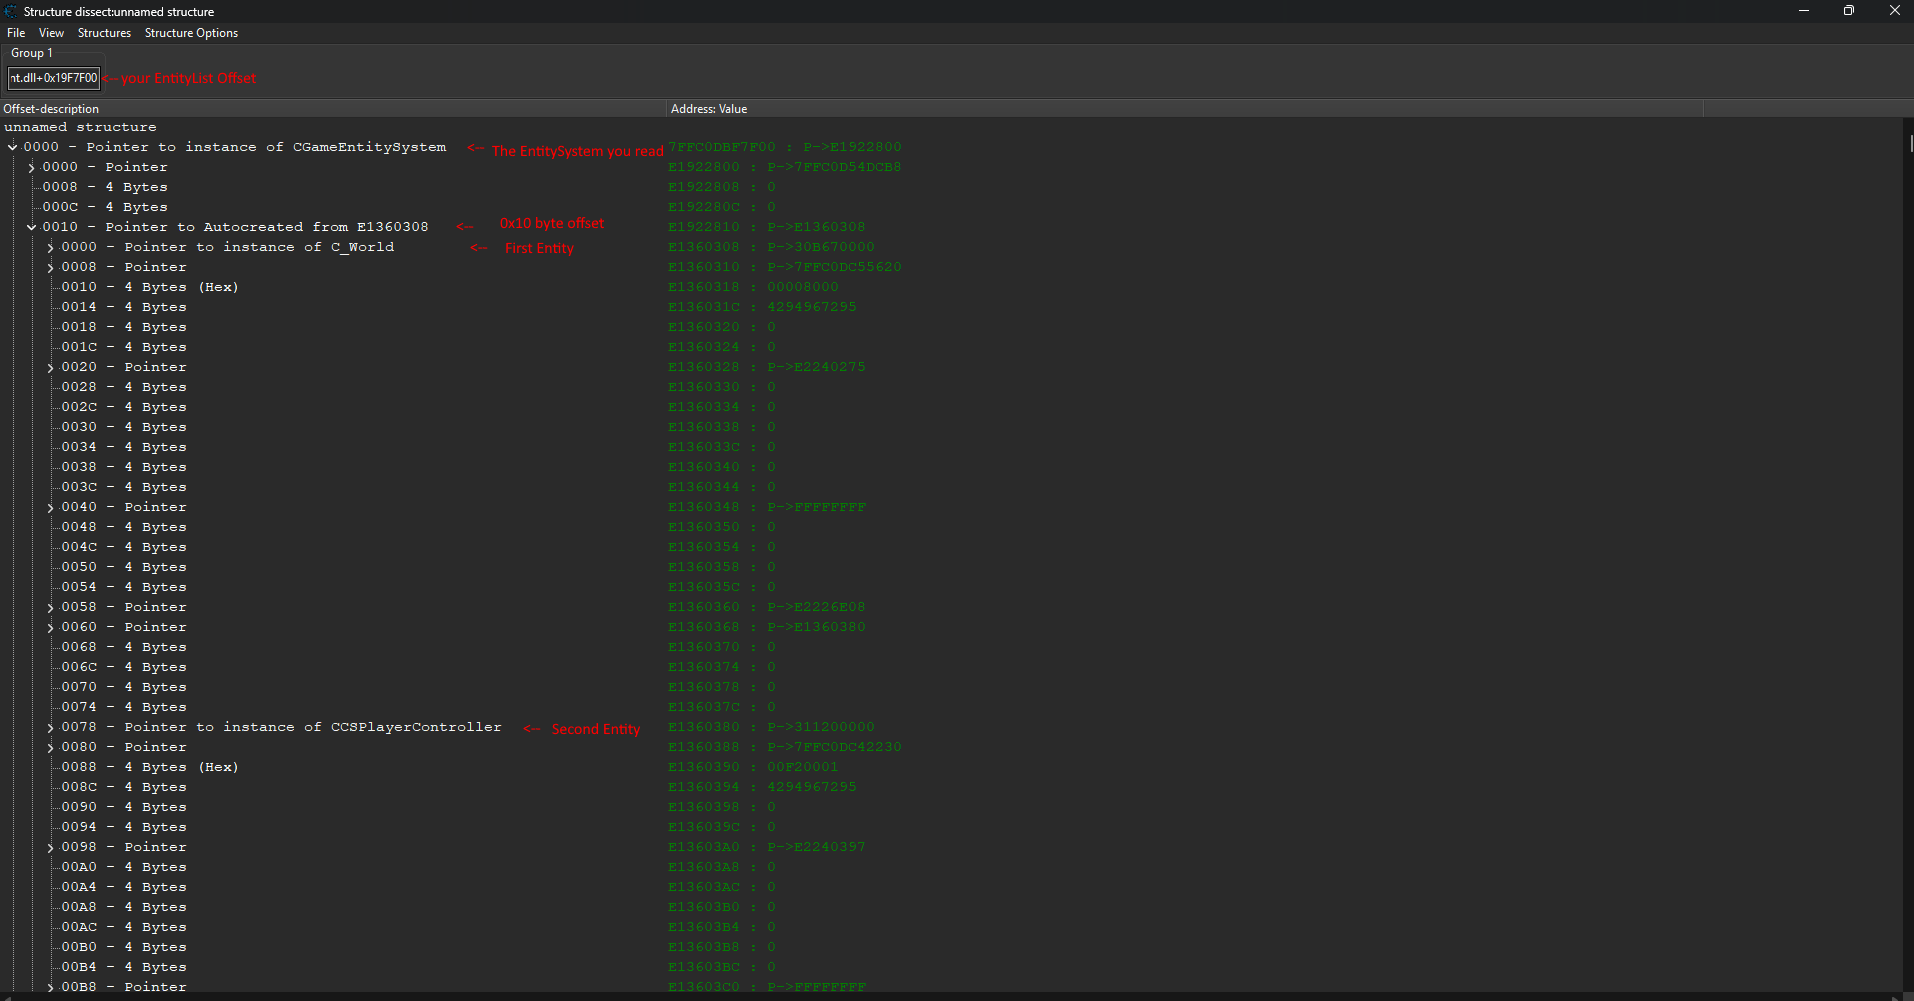
\includegraphics[width=1\linewidth]{images/al1gn_reclass_uc.png}
\end{frame}


\begin{frame}
    \frametitle{Feature: Chams \& Internal Material Injection}
    To implement Chams, we reverse engineered one of CS2’s internal material files to understand its structure.
    \vspace{0.4cm}
    \begin{itemize}
        \item \textbf{Material Discovery:} We decrypted and analyzed a material from Valve's asset system (suspected format: \texttt{.vk3}) dumped from memory.
    \end{itemize}
\end{frame}

\begin{frame}[plain]
    \begin{center}
        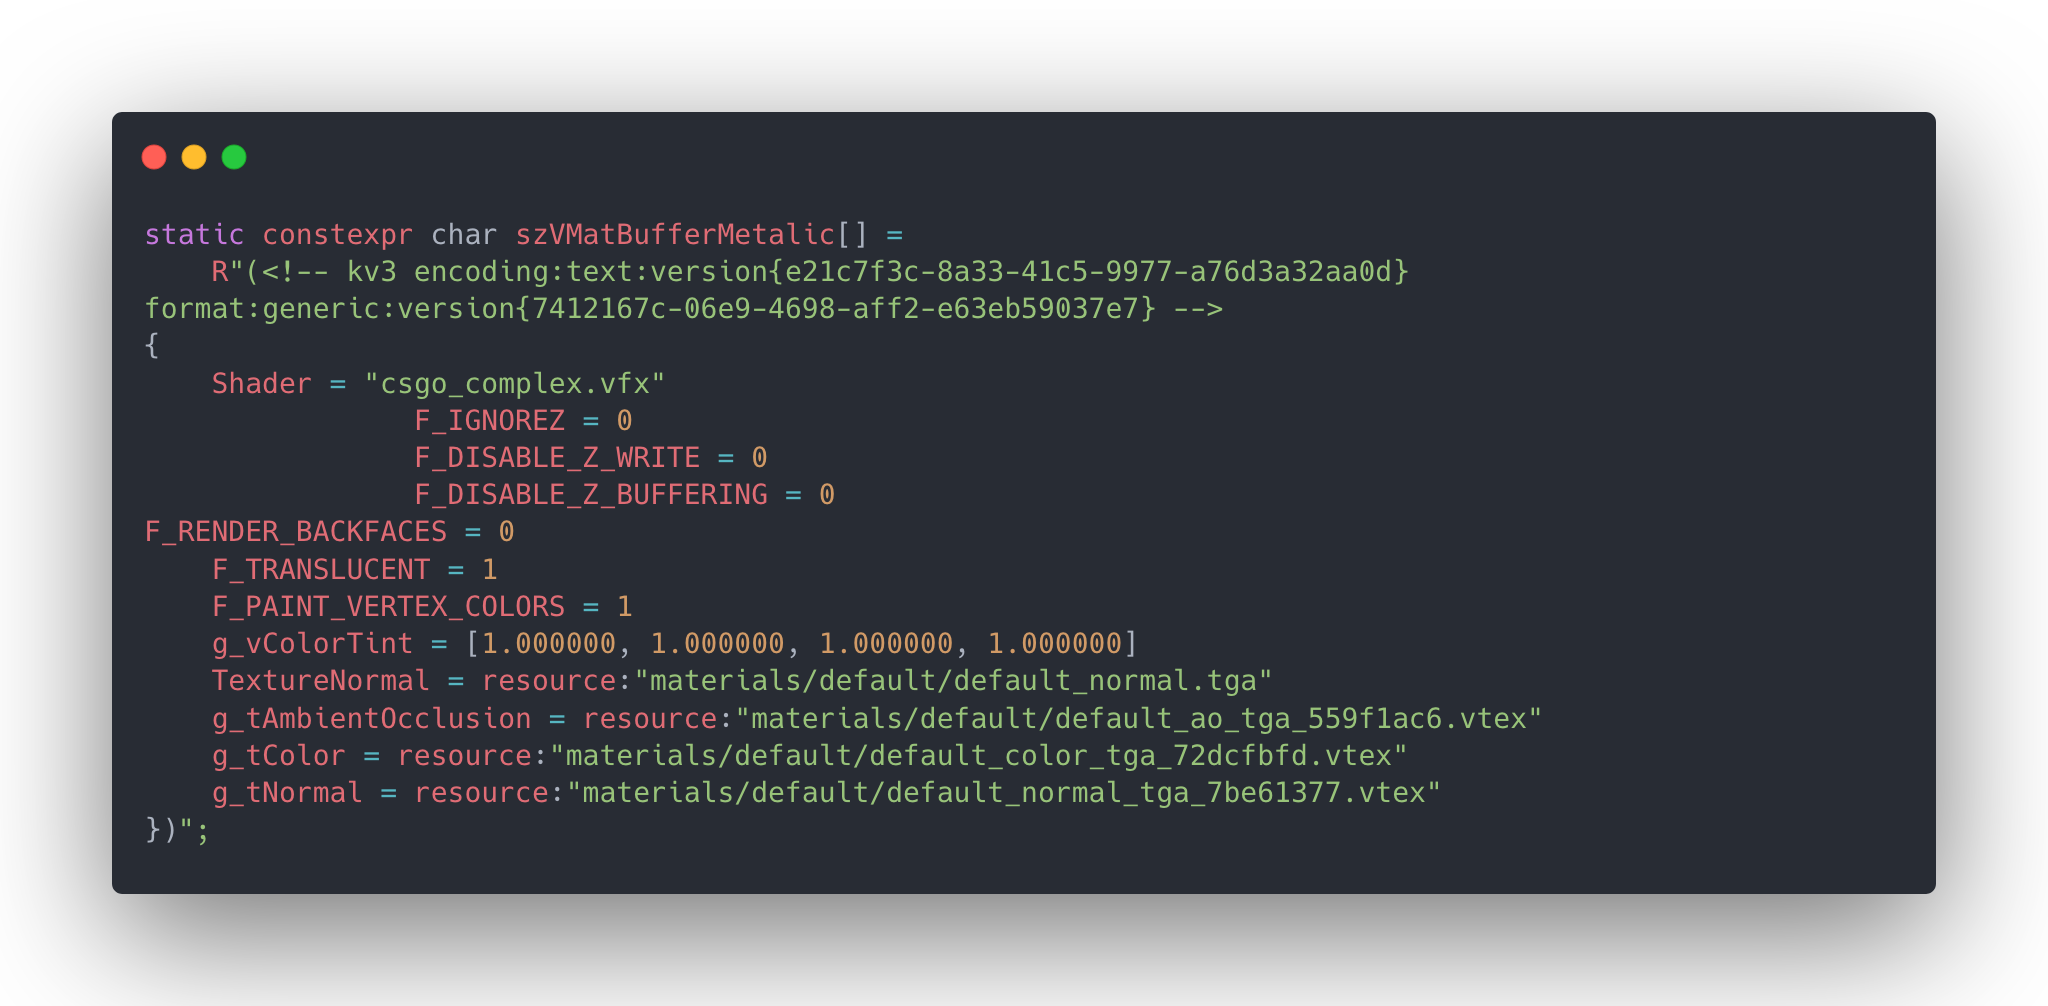
\includegraphics[width=\linewidth,height=\textheight,keepaspectratio]{images/carbon.png}
    \end{center}
\end{frame}

\begin{frame}
    \frametitle{Feature: Chams \& Internal Material Injection}
    To implement Chams, we reverse engineered one of CS2’s internal material files to understand its structure.
    \vspace{0.4cm}
    \begin{itemize}
        \item \textbf{Material Discovery:} We decrypted and analyzed a material from Valve's asset system (suspected format: \texttt{.vk3}) dumped from memory.
        \item \textbf{Function Hooks:} We hooked two internal engine functions: one responsible for material creation, another for rendering passes.
        \pause
        \item \textbf{Selective Injection:} By filtering the render queue, we applied our custom material only to specific models (e.g. \textbf{C\_CSPlayerPawn, C\_CSWeapon}).
    \end{itemize}
\end{frame}

% --- Visual Examples: Chams Materials ---
\begin{frame}
    \frametitle{Visual Examples: Chams Materials}        
    \includegraphics[width=1\linewidth]{../Master Thesis Template/images/chams/chams_demo/20250608210234_1.jpg}
\end{frame}

\begin{frame}
    \frametitle{Visual Examples: Chams Materials}        
    \includegraphics[width=1\linewidth]{../Master Thesis Template/images/chams/chams_demo/20250608210300_1.jpg}
\end{frame}

\begin{frame}
    \frametitle{Visual Examples: Chams Materials}        
    \includegraphics[width=1\linewidth]{../Master Thesis Template/images/chams/chams_demo/20250608210422_1.jpg}
\end{frame}

\begin{frame}
    \frametitle{Visual Examples: Chams Materials}        
    \includegraphics[width=1\linewidth]{../Master Thesis Template/images/chams/chams_demo/20250608210427_1.jpg}
\end{frame}


% --- NEW: Bone ESP: Skeleton Rendering via Bone Structures ---
\begin{frame}
    \frametitle{Bone ESP: Skeleton Rendering via Bone Structures}
    During our reverse engineering efforts, we located the in-memory structure used by CS2 to store bone positions for each player model.
    \vspace{0.4cm}
    \begin{itemize}
        \item \textbf{Bone Matrix Discovery:} The game maintains a matrix of bone positions indexed per entity, storing 3D coordinates for each joint.
        \pause
        \item \textbf{Bone Indices:} Once the matrix was located, we extracted the relevant joint coordinates and projected them into screen space.
        \pause
        \item \textbf{Skeleton Drawing:} We connected selected bones (e.g., head, spine, limbs) with lines to visually represent the player’s skeleton.
    \end{itemize}
\end{frame}


\begin{frame}
    \frametitle{Visual Examples: Bone Matrix}        
    \includegraphics[width=1\linewidth]{../Master Thesis Template/images/Bones/20250608220410_1.jpg}
\end{frame}


\begin{frame}
    \frametitle{Visual Examples: Skeleton}        
    \includegraphics[width=1\linewidth]{../Master Thesis Template/images/Bones/20250608220214_1.jpg}
\end{frame}

\begin{frame}
    \frametitle{Visual Examples: Skeleton \& Chams in a Real Match}        
    \includegraphics[width=1\linewidth]{../Master Thesis Template/images/Bones/20250608222558_1.jpg}
\end{frame}


\begin{frame}
    \frametitle{Visual Examples: Skeleton in a Real Match }        
    \includegraphics[width=1\linewidth]{../Master Thesis Template/images/Bones/20250608222549_1.jpg}
\end{frame}


\section{Reflections, Implications, and Future Work}

\begin{frame}
    \frametitle{Final Reflections}
    \begin{itemize}
        \item The cat-and-mouse dynamic between cheaters and anti-cheat systems reflects a fundamental aspect of human nature: \textbf{the relentless drive to win, by any means necessary}.
        \pause
        \item A single user, acting anonymously from home, can challenge and undermine the work of entire development teams and multi-million-dollar infrastructures.
        \begin{center}
            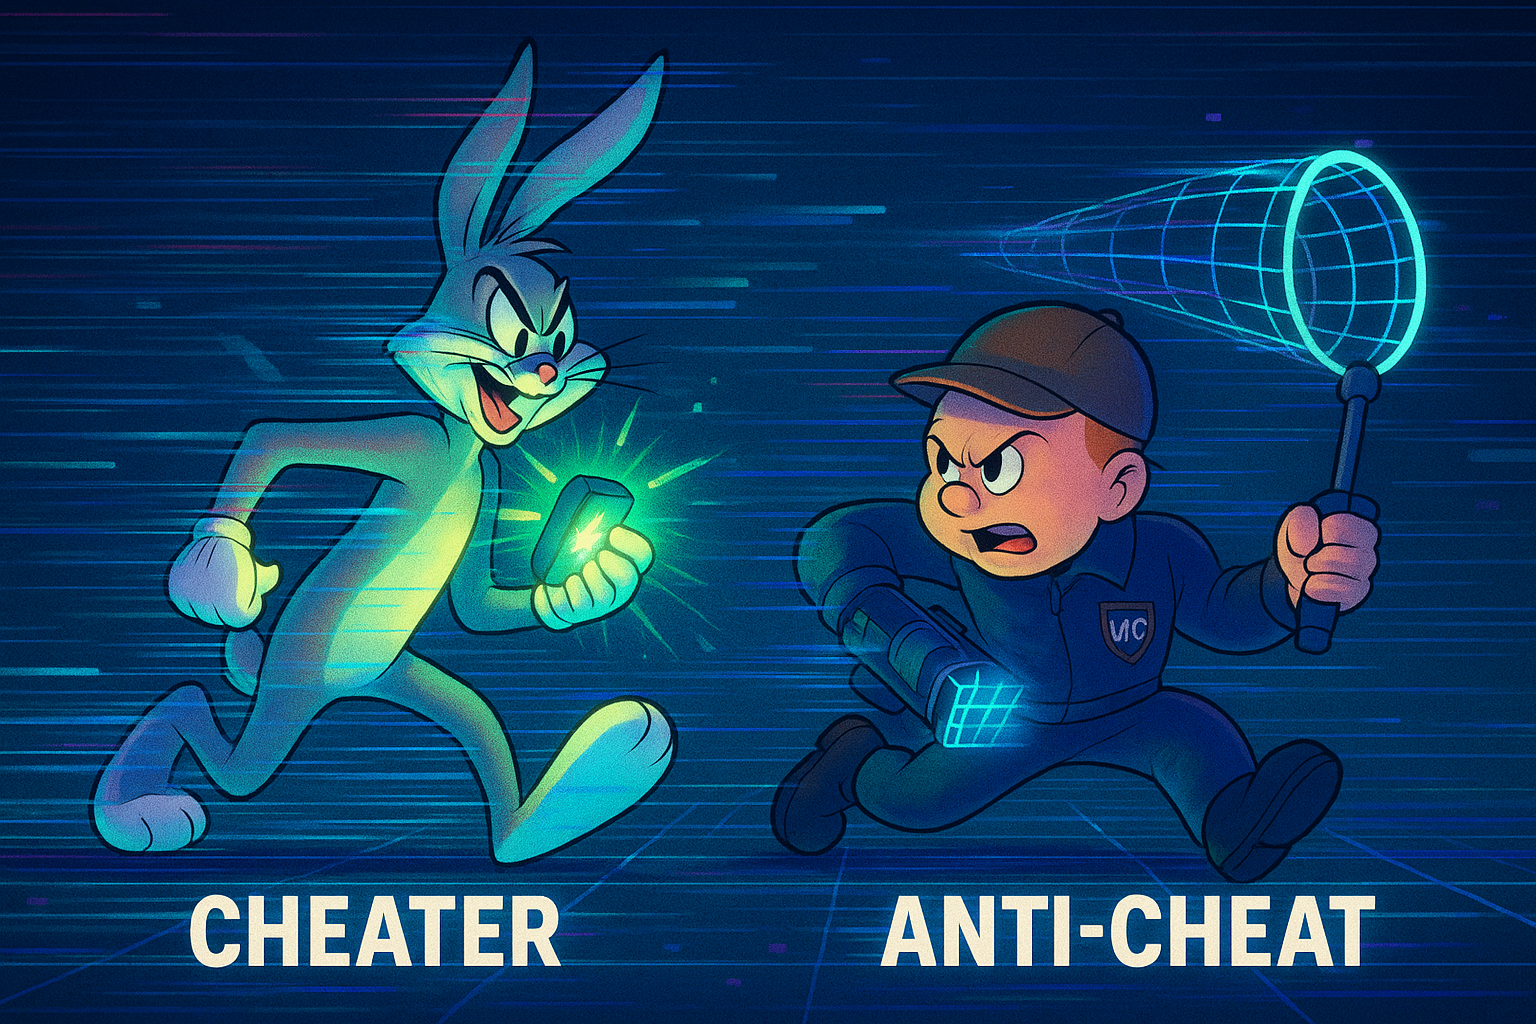
\includegraphics[width=0.5\linewidth]{images/cheater_anticheat.png}
        \end{center}
    \end{itemize}
\end{frame}

\begin{frame}
    \frametitle{Future Work and Research Directions}
    \begin{itemize}
        \item Integrate automated schema extraction and dynamic offset resolution for update resilience.
        \pause
        \item Design and test new stealth hooking methods, including hardware breakpoints and kernel-level injection.
        \pause
        \item Explore and implement hooks from the \textbf{Anti Cheat dumped modules}.
    \end{itemize}
\end{frame}

% --- Closing Questions Slide ---
\begin{frame}
    \frametitle{Questions}
    \begin{center}
        \Huge Thank you for your attention!\\[1em]
        \Large Any questions?
    \end{center}
\end{frame}

\end{document}
